\documentclass{article}
\usepackage{titlesec}
\usepackage[dotinlabels]{titletoc}
\usepackage[utf8]{inputenc}
\usepackage[russian]{babel}
\usepackage[a4paper, left=1.5cm, right=1.5cm, top=1cm, bottom=1cm]{geometry}
\usepackage[unicode, pdftex]{hyperref}
\setlength\parindent{0pt}
\pagenumbering{gobble}
\usepackage{caption} 
\captionsetup[table]{skip=5pt}
\usepackage{graphicx}
\usepackage{float}

\begin{document}

\begin{minipage}{0.62\textwidth}
    \begin{center}
        Санкт-Петербургский национальный исследовательский университет \\
        информационных технологий, механики и оптики \\
        УЧЕБНЫЙ ЦЕНТР ОБЩЕЙ ФИЗИКИ ФТФ
    \end{center}
\end{minipage}
\hfill
\begin{minipage}{0.38\textwidth}
    \centering
    \begin{figure}[H]
    
\includegraphics[width=\textwidth]{logo.png}
    \end{figure}
\end{minipage}

\rule{\textwidth}{1pt} \\

\begin{minipage}{0.16\textwidth}
        Группа \hrulefill\\
        Студент \hrulefill\\
        Преподаватель \hrulefill
\end{minipage}%
\begin{minipage}{0.25\textwidth}
        K3222\hrulefill\\
        Бевз Т.А.\hrulefill\\
        Соломонов А.И.\hrulefill
\end{minipage}
\hfill
\begin{minipage}{0.47\textwidth}
        К работе допущен \hrulefill\\
        Работа выполнена \hrulefill\\
        Отчёт принят \hrulefill
\end{minipage}
\begin{center}
    \textbf{\huge Рабочий протокол и отчет по \\
    лабораторной работе № 4.04}
\end{center}
\begin{minipage}{1\textwidth}
        \hrulefill\\
        \Large\textbf{Определение показателя преломления стеклянной пластины интерференционным методом}\hrulefill
\end{minipage}
\section{Цель работы}
\begin{enumerate}
     Определение показателя преломления стеклянной пластины с помощью интерференционной картины полос равного наклона и расчет порядка интерференции для центра картины.
\end{enumerate}

\section{Задачи, решаемые при выполнении работы}
\begin{enumerate}
    \item Определение координат минимумов интерференционных колец.
    \item Определение показателя преломления пластины.
    \item Измерение толщины пластины.
\end{enumerate}

\section{Объект исследования}
Плоскопараллельная пластина, интерференционная картина.
\section{Метод экспериментального исследования}
Физический эксперимент.
\section{Рабочие формулы и исходные данные}
\begin{equation}
 n = \frac{d(D^{2}_{2}-D^{2}_{1})}{16L^{2}\lambda \Delta m} - \textit{Показатель преломления материала плоскопараллельной пластины.}
 \label{eq:ref1}
\end{equation}
Где $d$ - толщина пластины, $D_{1}$, $D_{2}$ - диаметры колец с разностью порядка $\Delta m$ = 3, $L$ - расстояние между экраном и пластиной, $\lambda$ - длина волны
\begin{equation}
 \Delta_{z}=\sqrt{(\frac{\partial f}{\partial a}\Delta_{a})^2 + (\frac{\partial f}{\partial b}\Delta_{b})^2 + (\frac{\partial f}{\partial c}\Delta_{c})^2 + ...} - \textit{Погрешность искомой величины z как функции погрешностей прямо измеренных величин.}
 \label{eq:ref2}
\end{equation}
Где $\frac{\partial f}{\partial a}$; $\frac{\partial f}{\partial b}$; $\frac{\partial f}{\partial c}$; ... – частные производные искомой функции z
\begin{equation}
 m = \frac{2dn}{\lambda} - \textit{порядок интерференции в центре картины.}
 \label{eq:ref3}
\end{equation}
\newpage
\section{Измерительные приборы}
\begin{table}[h]
    \centering
    \bgroup
    \def\arraystretch{1.2}
    \begin{tabular}{|c|c|c|c|}
        \hline
        Наименоване & Тип прибора & Используемый диапазон & Погрешность \\
        \hline
        Шкала на оптическом рельсе & Аналоговый & $0-100$ см. & $0.1$ см. \\
        \hline
        Шкала на экране & Аналоговый & $-4 - 4$ см. & $0.1$ см. \\
        \hline
    \end{tabular}
    \egroup
    \caption{Измерительные приборы} 
\end{table}
\section{Схема установки}
\begin{figure}[h!]
    \begin{center}
    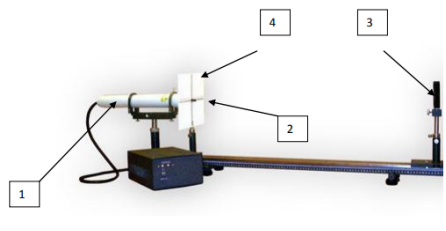
\includegraphics[width=0.6\textwidth]{scheme.png}
    \caption{Вид экспериментальной установки. 1 – лазер, 2 – микрообъектив, 3 – плоскопараллельная пластина, 4 – экран.}
    \label{fig:scheme}    
    \end{center}
\end{figure}
\section{Ход работы}
\begin{itemize}
  \item Для обработки результатов лабораторной работы было необходимо измерить растояние от плоскопараллельной пластины до микрообъектива $L = 78.8$ см. Также определить координаты пересечения с вертикальной и горизонтальной осями на экране у 7-8 темных расположенных подряд интерференционных колец. Результаты измерений представлены в таблице №2.
  \item Далее для каждого измерения были расчитаны диаметры последовательных колец. Вычисления также представлены в таблице №2.
  \item Из расчитанных ранее диаметров были выбраны пять пар, которые отличаются по порядку интерференции на 3. Для каждой пары были расчитаны $D^{2}_{2}-D^{1}_{2}$ и их усредненное значение <$D^{2}_{2}-D^{1}_{2}$> = $0.0018$ см$^{2}$.
  \item После этого, было найдено значение показателя преломления пластины n при ее толщине $d = 15.82$ мм и длине волны излучения $\lambda = 632.82$ нм. $n = 1.55$. Также с помощью рекомендаций из пособия по обработке экспериментальных данных была найдена его погрешность $\Delta n = 0.09$ при помощи формулы (2).
  \item Наконец, стало возможным вычислить порядок интерференции в центре картины $m = 77555$. Также была определена его погрешность $\Delta m = 4640$.
\end{itemize}
\section{Результаты прямых измерений и их обработки}
\begin{table}[h]
    \centering
    \bgroup
    \def\arraystretch{1.4}
    \begin{tabular}{|c|c|c|c|c|c|}
        \hline
        № & $X_{1}$, см & $X_{2}$, см & $Y_{1}$, см & $Y_{2}$, см & $D$, см\\ \hline
        $ 1 $ & $ -1.1 $ & $ 0.7 $ & $ -1.1 $ & $ 0.8 $ & $ 1.85 $\\ \hline
        $ 2 $ & $ -1.8 $ & $ 1.4 $ & $ -1.7 $ & $ 1.4 $ & $ 3.15 $\\ \hline
        $ 3 $ & $ -1.8 $ & $ 1.8 $ & $ -2.1 $ & $ 1.9 $ & $ 3.80 $\\ \hline
        $ 4 $ & $ -2.2 $ & $ 2.1 $ & $ -2.4 $ & $ 2.2 $ & $ 4.45 $\\ \hline
        $ 5 $ & $ -2.5 $ & $ 2.5 $ & $ -2.8 $ & $ 2.5 $ & $ 5.15 $\\ \hline
        $ 6 $ & $ -3.1 $ & $ 2.7 $ & $ -3.0 $ & $ 2.8 $ & $ 5.80 $\\ \hline
        $ 7 $ & $ -3.3 $ & $ 3.0 $ & $ -3.3 $ & $ 3.0 $ & $ 6.30 $\\ \hline
        $ 8 $ & $ -3.5 $ & $ 3.4 $ & $ -3.5 $ & $ 3.3 $ & $ 6.85 $\\ \hline
    \end{tabular}
    \egroup
    \caption{Координаты пересечения колец с горизонтальной и вертикальной осями.} 
\end{table}
\newpage
\section{Окончательные результаты}
\begin{enumerate}
    \item Показатель преломления пластины: $n = (1.55 \pm 0.09 )$; $\varepsilon_{n} = 6\%$  
    \item Порядок интерференции в центре картины: $m = (78 \pm 5 )\cdot 10^{3}$; $\varepsilon_{m} = 6\%$  
\end{enumerate}
\newpage
\section{Вывод}
Входе работы была был найден коэффициент преломления линзы путём создания и исследования интерференционной картины, созданной при помощи лазера, а также найден порядок интерференции в центре картины. Погрешности измерений объясняются погрешностями приборов. Показатель преломления различных видов стекол варьируетя от 1,44 до 1,79 - из этого можно сделать вывод, что полученный в результате выполнения лабораторной работы показатель $1.55 \pm 0.09$ имеет место быть.
\end{document}
